The idea behind patterns and sequences was to give a better insight into how the matrix is traversed.\newline
Consider the following example of accesses to a matrix:\newline
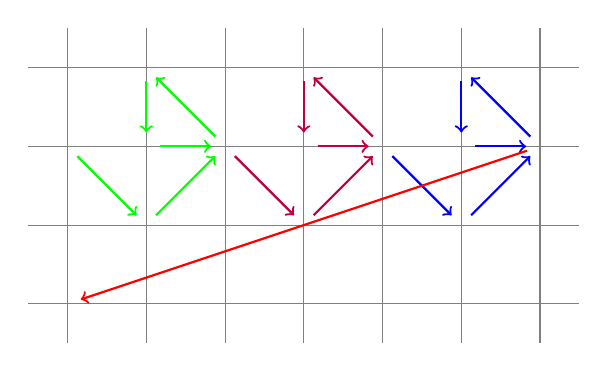
\begin{tikzpicture}
	\tikzstyle{accarrw} = [draw,->,thick, shorten <=5, shorten >=5]
	\draw [color=gray] (-0.5,-3.5) grid (6.5,0.5);
	\foreach \i/\c in {0/green, 1/purple, 2/blue} {
		\draw [accarrw,\c] ({0+\i*2},-1) -- ({1+\i*2},-2);
		\draw [accarrw,\c] ({1+\i*2},-2) -- ({2+\i*2},-1);
		\draw [accarrw,\c] ({2+\i*2},-1) -- ({1+\i*2},-0);
		\draw [accarrw,\c] ({1+\i*2},-0) -- ({1+\i*2},-1);
		\draw [accarrw,\c] ({1+\i*2},-1) -- ({2+\i*2},-1);
	}
	\draw [accarrw,red,bend left] (6,-1) -- (0,-3);
\end{tikzpicture}\newline
The green, purple and blue parts would each be considered an occurrence of the pattern (1,1),(1,-1),(-1,1),(0,1),(1,0). A pattern however does not know anything about which access is first or last, it only states that there is a short series of accesses that repeats.\newline
The three consecutive occurences of the pattern are considered a sequence. In this case, it's a sequence of length 3 with the next access (-6,2). The fact how often a sequence with these specifics is detected is counted by mctracer. Information that is not collected is; where the sequence was found (neither in terms of time or localization on the matrix) and which access of it's pattern was last (usually, it's the last access, but that isn't always certain).
